%%=====================================================================
%% INTRODUÇÃO: contexto, problema, conjugado da hélice, objetivos
%%=====================================================================
\begin{frame}{Albatroz Aerodesign}
  \begin{columns}[c]
    \begin{column}{0.42\textwidth}
      \begin{itemize}
        \item Competição SAE Brasil Aerodesign
        \item Motor BLDC obrigatório
        \item Propulsão define a carga útil
      \end{itemize}
    \end{column}
    \begin{column}{0.58\textwidth}
      \centering
      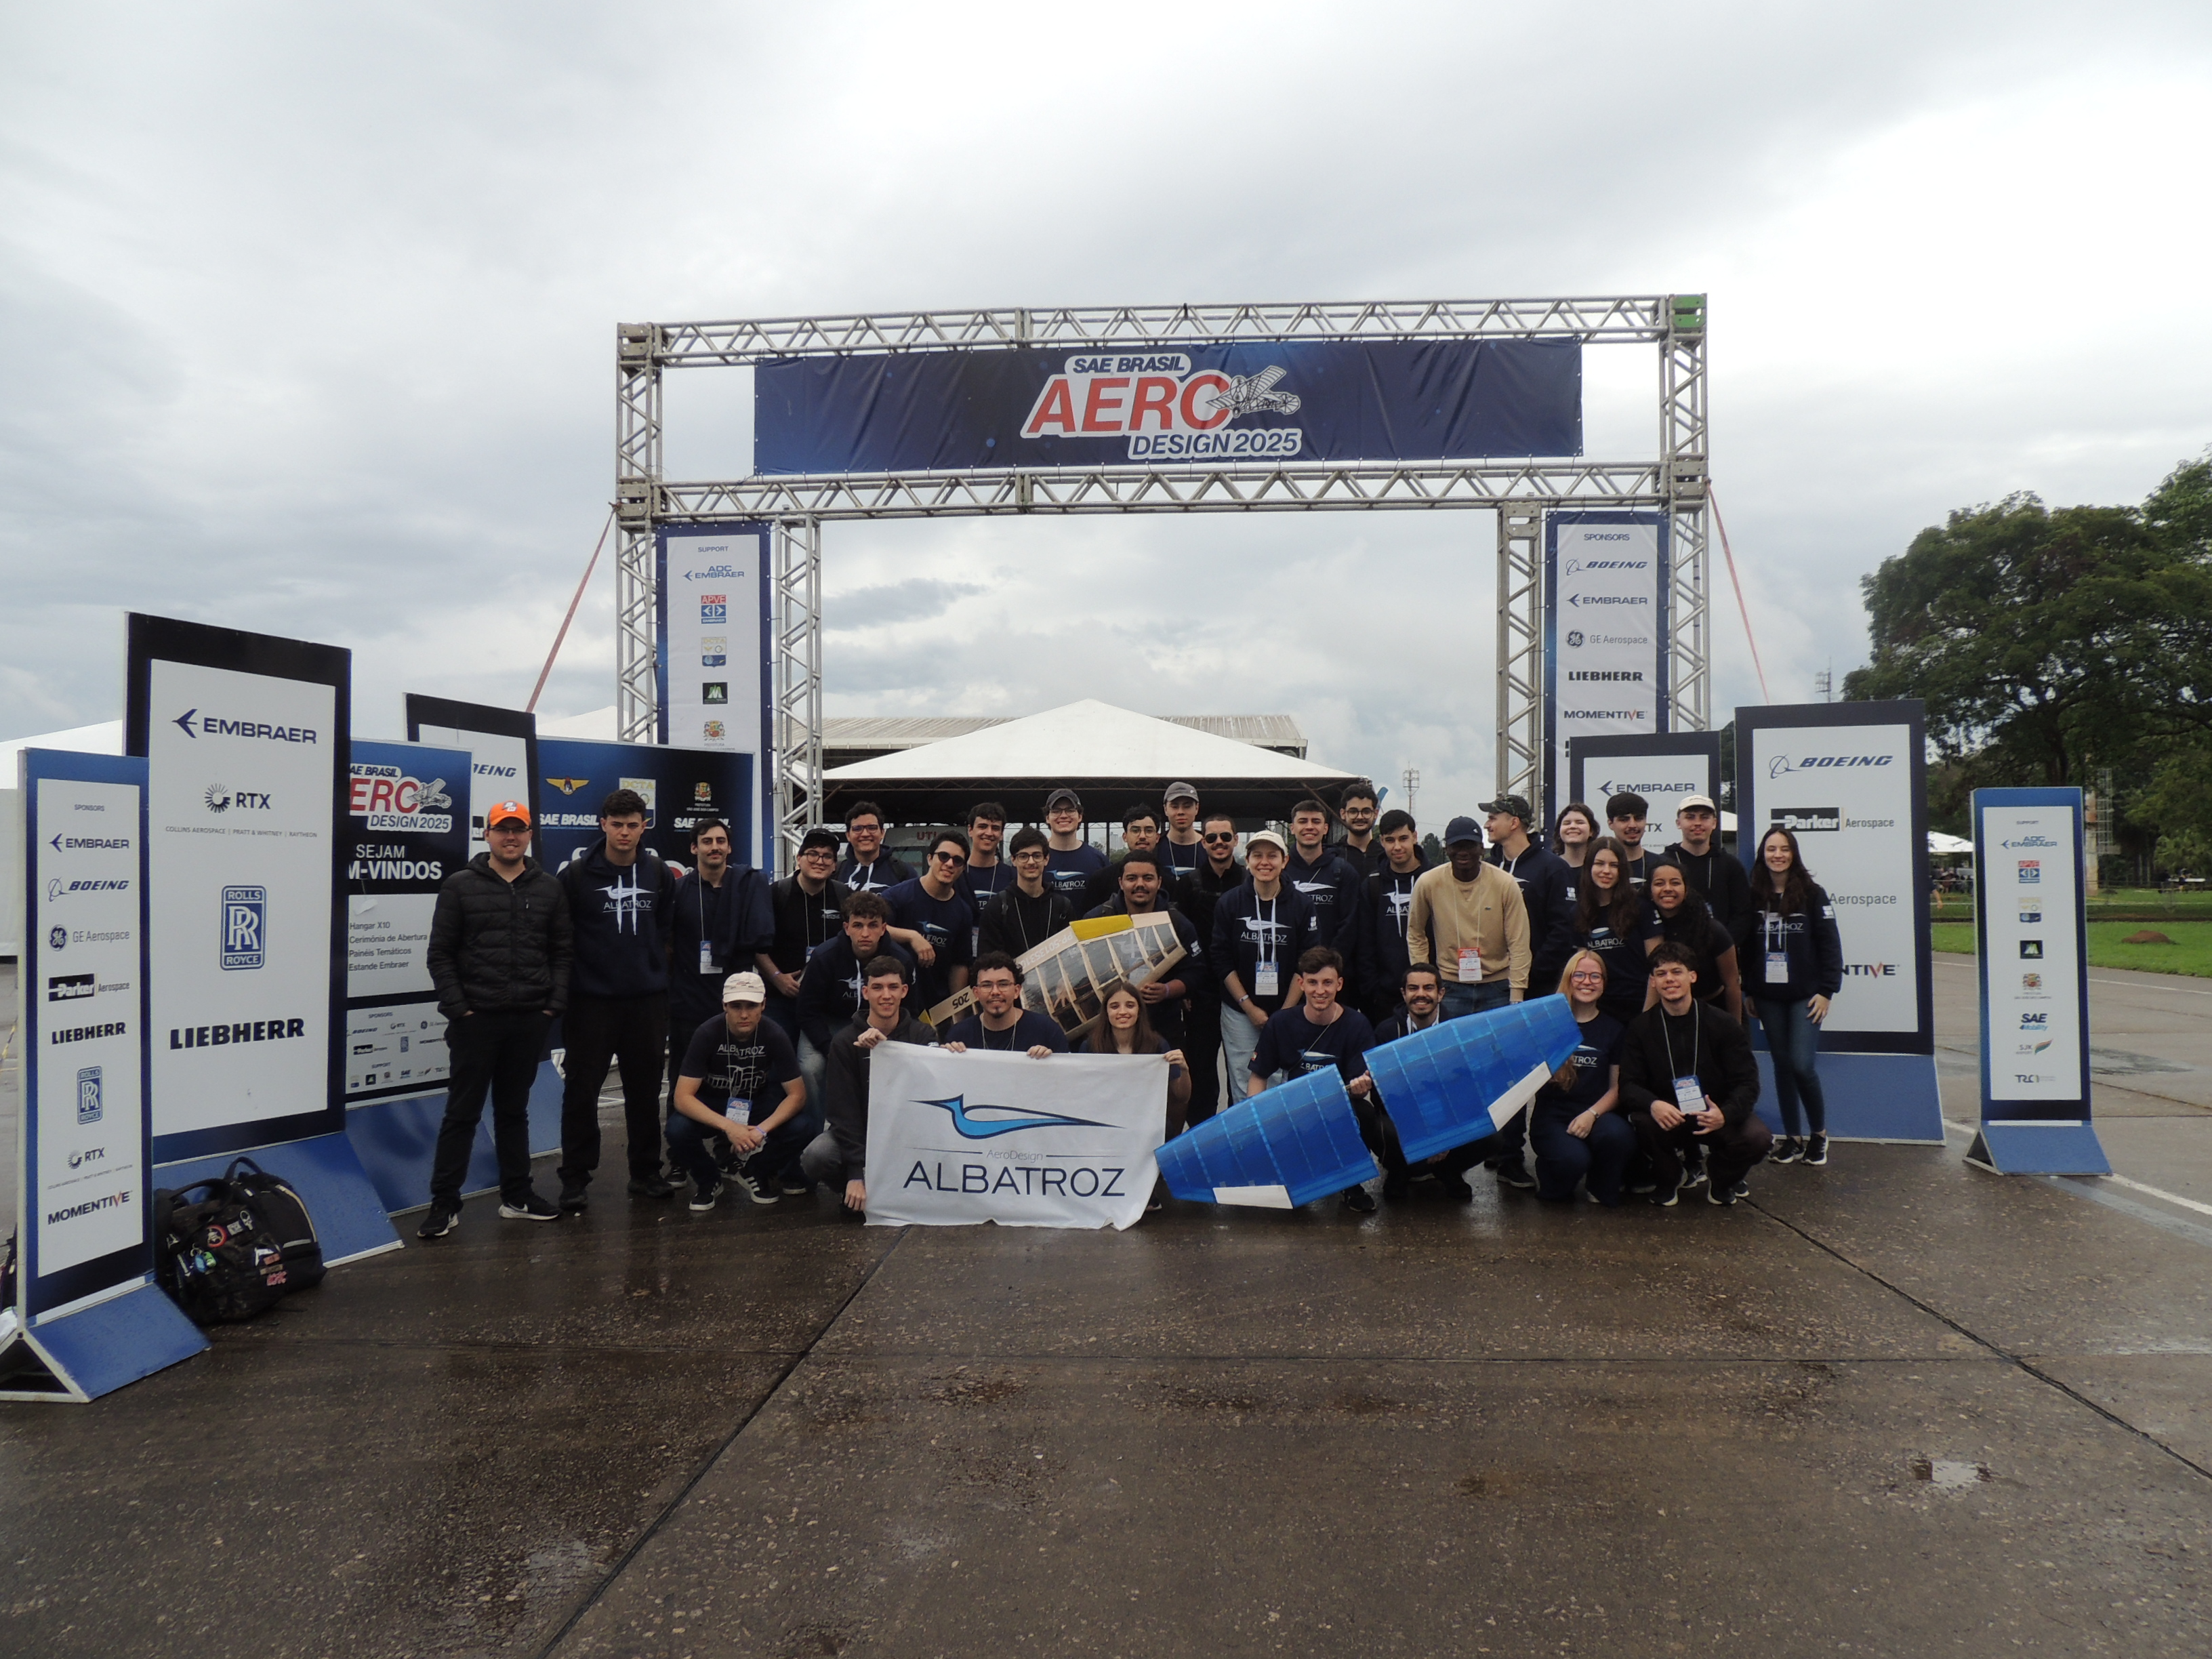
\includegraphics[width=\linewidth]{Introducao/DSCN3474.JPG}
      \fonte[Equipe Albatroz; SAE Brasil (2024)]
    \end{column}
  \end{columns}
\end{frame}

\begin{frame}{Ensaios descentralizados}
  \begin{columns}[c]
    \begin{column}{0.4\textwidth}
      \centering
      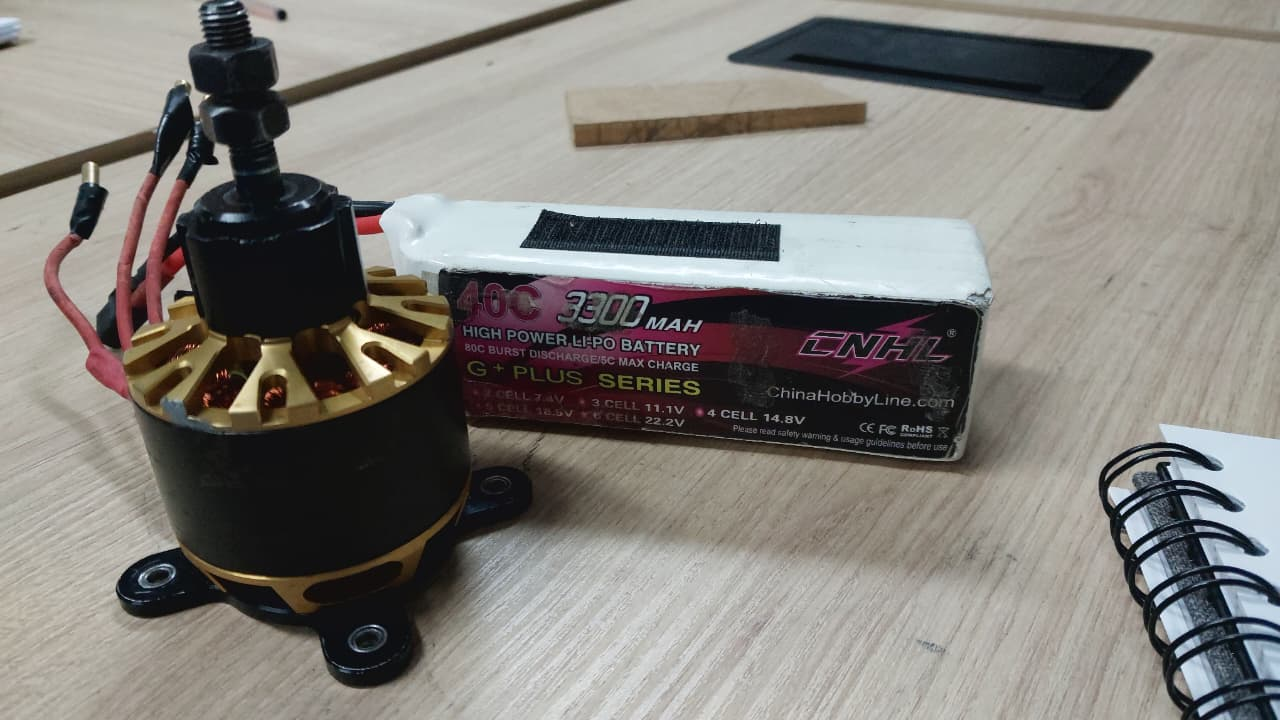
\includegraphics[height=0.5\textheight]{Metodologia/Motor_batata.jpeg}\\[0.3em]
      {\small Motor e bateria}
    \end{column}
    \begin{column}{0.6\textwidth}
      \centering
      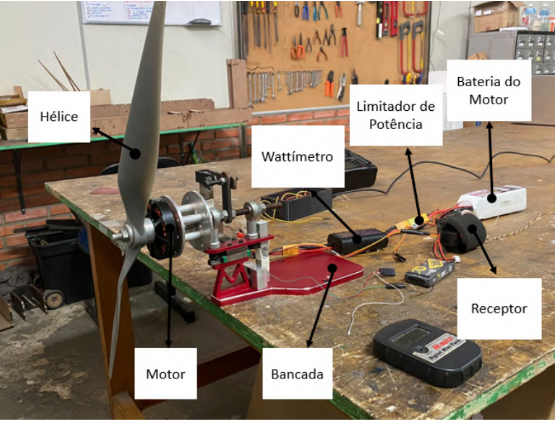
\includegraphics[height=0.5\textheight]{Introducao/BancadaDesempenho.png}\\[0.3em]
      {\small Bancada atual}
    \end{column}
  \end{columns}
  \destaque{Sem medida direta de rotação e torque: só estimativas.}
  \fonte[Autor; Souza e Veber (2023); Costa (2021)]
\end{frame}

\begin{frame}{Conjugado da hélice}
  \[ Q = C_Q\,\rho\,n^2 D^5 \]
  \begin{columns}[c]
    \begin{column}{0.5\textwidth}
      \centering
      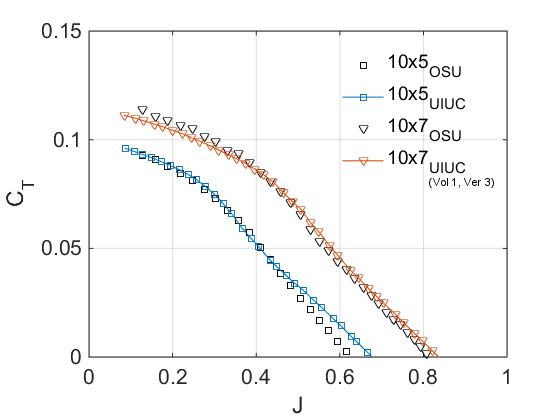
\includegraphics[height=0.5\textheight]{Revisao/Selig_propeller_data_ct.png}
    \end{column}
    \begin{column}{0.5\textwidth}
      \centering
      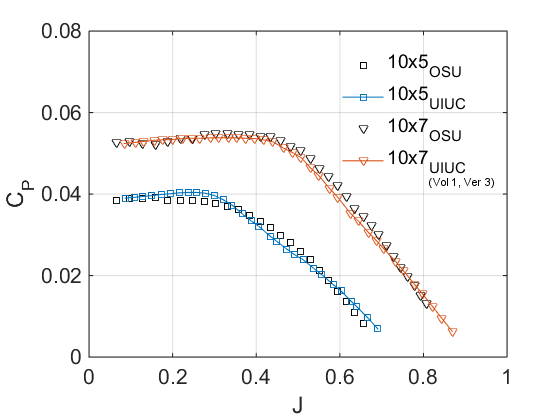
\includegraphics[height=0.5\textheight]{Revisao/Selig_propeller_data_cp.png}
    \end{column}
  \end{columns}
  \fonte[McCrink e Gregory (2015); McCormick (1995)]
\end{frame}

\begin{frame}{Torque define o envelope}
  \begin{columns}[c]
    \begin{column}{0.36\textwidth}
      Hélices de referência
      \begin{itemize}
        \item APC 15x6E
        \item APC 17x10E
      \end{itemize}
      \vspace{0.5em}
      Simuladas com o catálogo e ensaiadas em bancada
    \end{column}
    \begin{column}{0.64\textwidth}
      \centering
      \tikzfig{1}{0.7}{helice_ponto_op}
      \fonte[Autor; APC Propellers (2026); Brandt et al.\ (2015)]
    \end{column}
  \end{columns}
\end{frame}

\begin{frame}{Objetivos}
  \destaque{Desenvolver um sistema integrado de aquisição de dados,
            adaptando a bancada de ensaios motopropulsores da equipe.}

  \vspace{0.6em}
  \begin{itemize}
    \item Sistema de medição do motor BLDC
    \item Modelo do motor e observador de estados
    \item Medição aerodinâmica da hélice
    \item Rede Ethernet entre os nós e o supervisório
    \item Software de supervisão em Python
  \end{itemize}
\end{frame}
